\chapter*{About the author}
\addcontentsline{toc}{chapter}{About the author}

\begin{wrapfigure}{r}{0.5\textwidth}
    \vspace{-20pt}
    \begin{center}
        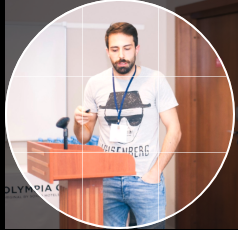
\includegraphics[width=0.48\textwidth]{images/me_linkedin}
    \end{center}
    %\vspace{-20pt}
    %\caption{A gull}
    \vspace{-15pt}
  \end{wrapfigure}

Davide Spataro was born and brought up in Southern Italy. He discovered a love of coding early on and, after attending a high school that focused on humanities, he moved to the University of Calabria in 2008 where he studied and worked for 3 years collaborating with researchers of the Department of Mathematics and Computer Science on the modelling and simulation of complex natural systems. He obtained his BSc in Computer Science in 2011, his MSc (summa cum laude) in 2014 and, in 2018, he successfully defended his Ph.D. thesis with the title: \quotes{Acceleration of numerical regular grid methods on manycore systems}. He has worked as a Software Engineer at ASML working on TWINSCAN photolitography systems and at DEGIRO as senior software enginner.
He has been involved in programming competitions since age 12 and is passionate about  \CC, parallel programming and GPGPU. When absolutely forced to do something other than think about coding problems, Davide can be found either arguing with gravity on a racing bike, paddling in the Mediterranean, listening to or playing classical and jazz piano, or drinking vast amounts of coffee. It's probably fair to say he thinks about coding when doing these things too. 
